\section{Trabajos previos}
El c\'omputo consciente del contexto es un t\'ermino discutido por primera vez en el trabajo de Schilit y Theimer \cite{schillit1994disseminating} como software que se adapta de acuerdo al contexto, esto limita la definici\'on a aplicaciones que son informadas sobre el contexto y se adaptan a \'el, no dejando en claro qu\'e tipo de adaptaci\'on es la que realiza. En investigaciones m\'as recientes, Dey \cite{dey2001conceptual}, define computaci\'on consciente del contexto como un sistema que usa el contexto para proporcionar informaci\'on relevante y/o servicios al usuario, donde la relevancia depende de la tarea del usuario. La definici\'on de Dey se puede ver reflejada en el ejemplo del sistema gu\'ia de turistas, donde la informaci\'on dada por el sistema es de inter\'es para los usuarios y la actividad que realizan, como por ejemplo, notificar de eventos pr\'oximos, o recomendar actividades o lugares a los turistas. En el caso de los videojuegos, el sistema ejecutar\'a instrucciones para ir aumentando la dificultad o el nivel del juego conforme el usuario va incrementando su habilidad, esto cumple la segunda propiedad de la definici\'on de Dey que es ejecutar comandos para adaptarse al contexto.

Una arquitectura consciente del contexto debe de cumplir con las siguientes caracter\'isticas\cite{dey1999architecture}:

\begin{itemize}
\item Acceso distribuido a la informaci\'on contextual.
\item Soporte multiplataforma y multilenguaje.
\item Interpretaci\'on contextual.
\item Agregaci\'on de informaci\'on contextual.
\item Independencia y persistencia de widgets contextuales.
\item Almacenamiento hist\'orico de la informaci\'on contextual.
\end{itemize}

Adem\'as de estas caracter\'isticas se deben de cumplir los siguientes requerimientos\cite{el2011distributed}: una formalizaci\'on de contexto para delimitar los datos contextuales  y facilitar la distinci\'on  de par\'ametros contextuales, una categorizaci\'on de datos para reducir la complejidad de su manutenci\'on; el segundo requerimiento son reglas de adaptaci\'on: la adaptaci\'on del contexto debe ser vista como un conjunto de reglas que controlan y anticipan el cambio de contexto que puede ocurrir en el ambiente, por lo tanto en la construcci\'on de reglas de adaptaci\'on, el n\'umero de par\'ametros contextuales es grande y as\'i, es evidente que no se pueden enumerar todas las posibles situaciones que van a ocurrir, es por esto que se requiere un m\'etodo para construir reglas de adaptaci\'on que pueda manejarla diversidad de posibles situaciones que se construyen en base de esos par\'ametros contextuales.

Muchas arquitecturas se han propuesto para poder soportar sistemas conscientes del contexto, la siguiente tabla hace una comparaci\'on de los elementos y capas de algunas arquitecturas conscientes del contexto, entre las cuales se encuentran la arquitectura base para el presente trabajo que usa un modelo contextual colaborativo clasificado en tres categor\'ias: elementos cohesivos, elementos interactivos y elementos afectivos. La arquitectura de Dey\cite{dey1999architecture}  usa widgets para la captura de datos contextuales y servicios de agregaci\'on de contexto as\'i como servicios de distribuci\'on y razonamiento contextual. En el marco de trabajo de Kamoun \cite{kamoun2012fadyrcos}  se reconfiguran servicios para adaptarlos a situaciones que cambian din\'amicamente. Decouchant \cite{decouchant2013adapting} divide su arquitectura en tres capas: la capa de espacio de trabajo, la de adaptaci\'on y la de detecci\'on de informaci\'on contextual. Guerman  \cite{guermah2013ontology} que propone una arquitectura orientada a sistemas de aprendizaje electr\'onico. En la figura \ref{cmp:fig} se comparan algunos elementos que poseen dichas arquitecturas, entre ellos se encuentran la presencia de capas como adquisici\'on, manejo y distribuci\'on de datos contextuales, persistencia de datos y su reuso, apoyo con v\'ias de comunicaci\'on, el uso de widgets como comunicadores entre el sistema y la arquitectura, manejo de sesiones, esquemas conceptuales de colaboraci\'on, agregaci\'on de datos y la representaci\'on de espacios de trabajo como parte de la arquitectura.

\begin{figure}[h!]
  \centering
    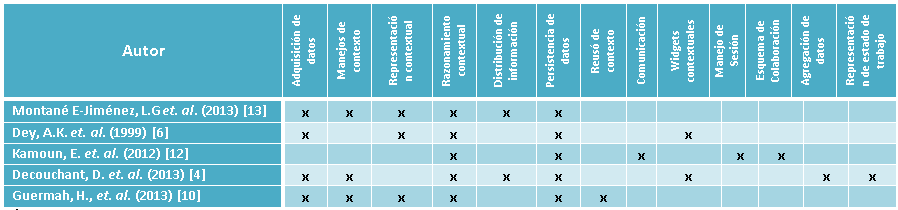
\includegraphics[scale=0.5]{images/comparaciones}
  \caption{Comparaci\'on de arquitecturas que soportan consciencia del contexto\cite{montane2013context}\cite{dey1999architecture}\cite{kamoun2012fadyrcos}\cite{decouchant2013adapting}\cite{guermah2013ontology}}
  \label{cmp:fig}
\end{figure}
